
%-----------------------------------------------------------------------
%中国科学: 数学 中文模板, 请直接用 LaTeX 编译
% SCIENTIA SINICA~~Mathematica
%-----------------------------------------------------------------------

\documentclass{SCIA2023cn}
%%%%%%%%%%%%%%%%%%%%%%%%%%%%%%%%%%%%%%%%%%%%%%%%%%%%%%%
%%% 作者附加的定义
%%% 常用环境已经加载好, 不需要重复加载
%%%%%%%%%%%%%%%%%%%%%%%%%%%%%%%%%%%%%%%%%%%%%%%%%%%%%%%

\DeclareMathOperator*{\esssup}{ess\,sup}
%%%%%%%%%%%%%%%%%%%%%%%%%%%%%%%%%%%%%%%%%%%%%%%%%%%%%%%
%%% 开始
%%%%%%%%%%%%%%%%%%%%%%%%%%%%%%%%%%%%%%%%%%%%%%%%%%%%%%%
%\def\dl{\displaystyle}
%\numberwithin{equation}{section}
%\newcommand{\upcite}[1]{\textsuperscript{\textsuperscript{\cite{#1}}}}

\newtheoremstyle{mystyle}{0pt}{0pt}{\normalfont}{1.82em}{\bf\heiti\color{blue}\zihao{5}}{}{1.29em}{}


\theoremstyle{mystyle}
\newtheorem{theorem}{定理}[section]
\newtheorem{definition}{定义}[section]
\newtheorem{lemma}{引理}[section]
\newtheorem{corollary}{推论}[section]
\newtheorem{proposition}{命题}[section]
\newtheorem{conjecture}{猜想}[section]
\newtheorem{remark}{注}[section]
\newtheorem{example}{例}[section]
\newtheorem{problem}{问题}[section]
\newtheorem{assumption}{假设}[section]
\newtheorem{conditions}{条件}[section]
\newtheorem{property}{性质}[section]

\begin{document}

%%%%%%%%%%%%%%%%%%%%%%%%%%%%%%%%%%%%%%%%%%%%%%%%%%%%%%%
%%% Authors do not modify the information below
%%% 作者不需要修改此处信息
%科学与技术前沿论坛
\ArticleType{论~~~文}%论~~~文
%\ArticleType{综~~~述}{}
%\SpecialTopic{自然科学基金项目进展专栏}%专题或专刊虚拟现实前沿技术专刊
%\SubTitle{献给XXX教授90 华诞}%专刊说明
%\Luntan{中国科学院学部\quad 科学与技术前沿论坛}
%\Year{2022}
%\Vol{52}
%\No{?}
\BeginPage{1}
%\DOI{10.1360/SSM-2022-XXXX}%doi号
%\ReceiveDate{2015--00--00}
%\AcceptDate{2015--00--00}
%\OnlineDate{2015--00--00}
%\ReceiveDate{2021-XX-XX} % 收稿日期
%\AcceptDate{2022-XX-XX} % 接受日期
%\OnlineDate{2022-03-XX} % 网络出版日期
%%%%%%%%%%%%%%%%%%%%%%%%%%%%%%%%%%%%%%%%%%%%%%%%%%%%%%%

\title{统计分析}{统计分析人权}

\entitle{Title}{Title for citation}%英文题目

\author[1]{张三三}{youxiang}{}%作者及邮箱
\author[2]{李四}{youxiang}{}%作者及邮箱
\author[1]{赵六}{youxiang}{$^*$}%通信作者请在相应作者后加*号
\enauthor[]{Sansan Zhang}{}%名前姓后,首字母大写其他小写
\enauthor[]{Si Li}{}
\enauthor[]{Liu Zhao}{}

\address[1.]{地址, 城市 000000;}%作者单位, 城市 邮编
\address[2.]{地址, 城市 000000}%作者单位, 城市 邮编
%\enaddress[1]{Address, City {\rm 000000}, Country}



\Foundation{国家自然科学基金(批准号: 1080000)资助项目}%基金及基金的批准号

\AuthorMark{张三三等}%第一作者等

%\AuthorCitation{姓名, 姓名}
\enAuthorCitation{Zhang S S, Li S, Zhao L}%引用条的作者姓名


\abstract{中文摘要(100--200字)中文摘要中文摘要中文摘要中文摘要中文摘要中文摘要中文摘要中文摘要中文摘要中文摘要中文摘要中文摘要中文摘要,
中文摘要中文摘要中文摘要中文摘要中文摘要中文摘要中文摘要中文摘要.
}%中文摘要

\enabstract{An abstract (100--200 words) is a summary of the content of the manuscript. It should briefly describe the research purpose, method, result and conclusion.
The extremely professional terms, special signals, figures, tables, chemical structural formula, and equations should be avoided here, and citation of references is not allowed.
}%英文摘要

\keywords{中文关键词\quad 中文关键\quad 中文关键}%关键词一般3~8个

\enkeywords{keyword1, keyword2, keyword3}%英文关键词3~8个

\MSC{60Fxx, 60Fxx, 60Axx}%主题分类号

\enMSC{60Fxx, 60Fxx, 60Axx}%主题分类号


\maketitle


%%%%%%%%%%%%%%%%%%%%%%%%%%%%%%%%下面为正文部分%%%%%%%%%%%%%%%%%%%%%%%%%%%%%%%%%%%%%%%%%%%%%%

%正文中图、表、公式、定理等需加标签\label{},引用时\ref{}
%正文中的概率、期望和方差需用白正体
%正文中的定理、引理等需用环境定义

\section{引言}
正文内容.

\begin{theorem}\label{theorem1.1}%需添加标签,后文引用定理时需用定理\ref{}格式
设$v$是二维不可压缩Navier-Stokes方程光滑的温和古代解, $w=\nabla\times v$是涡度. 若对所有的$t\in(-\infty,0)$ 一致成立
\begin{align}\label{w}%需添加标签,后文引用需用\ref{}格式
\lim_{|x|\rightarrow +\infty}|w(x,t)|=0,
\end{align}
则$w\equiv 0$并且$v$是调和的.
 \end{theorem}

\begin{theorem}\label{theorem1.2}
%\th{定理1.2}
设$v$是三维不可压缩轴对称Navier-Stokes方程具平凡角向速度($v_{\theta}=0$)时光滑的温和古代解, $w=\nabla\times v=w_{\theta}e_{\theta}$是涡度.
定义$\Omega=\frac{w_\theta}{r}$. 若对所有的$t\in(-\infty,0)$一致成立
%正文中的公式建议使用align, 不建议使用equation和eqnarray
\begin{align}\label{w2}
\lim_{r\rightarrow +\infty}|\Omega|=0,
\end{align}
则$w_\theta\equiv 0$并且$v$是调和的.先文后图, 图\ref{figure1} 正文正文正文正文正文正文.正文正文正文正文正文正文. 正文正文正文正文正文正文.正文正文正文正文正文正文.正文正文正文正文正文正文.正文正文正文正文正文正文.
 \end{theorem}

%%%%%%%%%%%%%%%%%图中的英文单词均需翻译成中文 %%%%%%%%%%%%%%%%%
\begin{figure}[!h]
 \centering
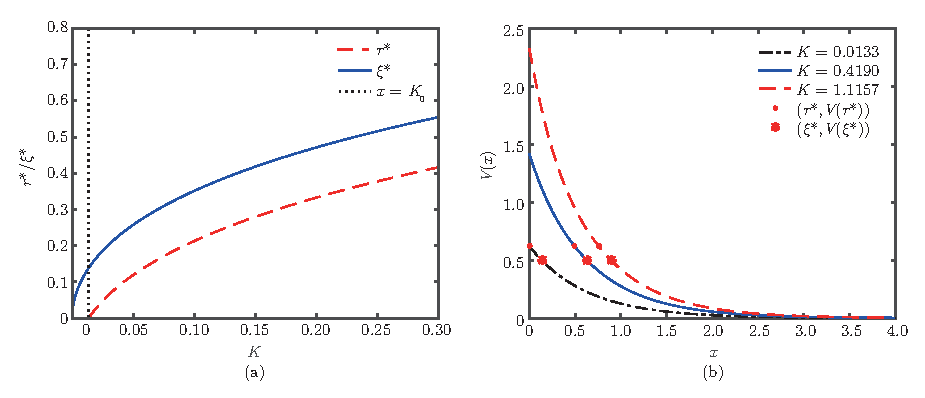
\includegraphics{t1.eps}\\
\cnenfigcaption{比例成本参数 $\bm{\kappa=0.8<1}$. (a) 固定成本参数 $\bm{K}$  对最优注资策略阈值 $\bm{r^*}$ 和 $\bm{\xi^*}$ 的影响; (b) 固定成本参数 $\bm{K}$  对值函数 $\bm{V(x)}$ 的影响}{}
\label{figure1}
\end{figure}

\begin{proof}
正文正文正文正文正文正文正文正文正文正文正文正文正文正文,
正文正文正文正文正文正文正文正文正文正文正文正文正文正文正文正文正文正文正文正文正文正文正文.
正文正文正文正文正文正文正文正文正文正文正文正文正文正文正文正文正文正文.
\end{proof}
事实上, 我们在文献\cite{1}中所用的方法表面上简单自然,正文正文正文正文正文正文.

先文后图, 图\ref{figure1} 正文正文正文正文正文正文, 而我们在文献\cite{1}
中的正文正文正文正文正文正文正文正文正文正文正文正文正文正文正文正文正文正文.
事实上, 我们在文献\cite{1} 中正文正文正文正文正文正文.


\section{一级标题}
先文后图,图\ref{figure1} 正文内容正文内容正文内容正文内容正文内容正文内容正文内容.

\subsection{二级标题}
正文正文正文正文正文正文.
\subsection{二级标题}
 由第2.1小节的证明思路可以看出, Liouville定理在证明中起到了关键作用. 公式(\ref{w}) 正文正文正文正文正文正文. 图\ref{figure1}正文正文正文正文正文正文.
 文献\cite{1} 提出了不可压缩Navier-Stokes方程古代解的Liouville定理的猜想, 即有界的温和古代解必为常数(定理\ref{theorem1.1}). 该文献证明了二维情形以及三维轴对称情形时的Liouville定理, 具体可分为以下几个结论.


  Chung 和 Erd\"os \upcite{1}正文内容正文内容正文内容正文内容正文内容正文内容正文内容.先文后表, 表\ref{tab1}正文内容.
  \begin{table}[!h]
  \centering
\cnentablecaption{表题}{}
\label{tab1}
\footnotesize
%\tabcolsep 49pt %space between two columns. 用于调整列间距
\begin{tabular}{cccccccc}
\toprule
  Title a & Title b & Title c & Title d \\   %%表中的英文单词均需翻译成中文
  \hline
  Aaa & Bbb & Ccc & Ddd\\
  Aaa & Bbb & Ccc & Ddd\\
  Aaa & Bbb & Ccc & Ddd\\
\bottomrule
\end{tabular}
\end{table}

\section{一级标题}
正文内容正文内容正文内容正文内容正文内容正文内容正文内容.


\Acknowledgements{此处可对审稿人以及给予过帮助的人表示感谢.}
%%%%%%%%%%%%%%%%%%%%%%%%%%%%%%%%%%%%%%%%%%%%%%%%%%%%%%%
%%% 补充材料说明
%%%%%%%%%%%%%%%%%%%%%%%%%%%%%%%%%%%%%%%%%%%%%%%%%%%%%%%
%\Supplements{补充材料.}

%%%%%%%%%%%%%%%%%%%%%参考文献格式要求%%%%%%%%%%%%%%%%%%%%%%%%%%%%%
%%% 参考文献, {}为引用的标签, 数字/字母均可
%%% 文中上标引用: \upcite{1,2}
%%% 文中正常引用: \cite{1,2}
%%%%%%%%%%%%%%%%%%%%%%%%%%%%%%参考文献部分%%%%%%%%%%%%%%%%%%%%%%%%%%%%%%%%%%%%%%%%%%%%
%正文中的文献平排需用\cite{}, 上角标用\upcite{}, 文献采用作者姓氏首字母顺序编号, 中文文献需同时提供相应的英文信息.
%每篇文献后,有doi号的,请补充doi
\begin{thebibliography}{99}  %%文后出现的参考文献在文中都必须引用

\bibitem{1} Chung K L, Erd\"os P. On the application of the Borel-Cantelli lemma. Trans Amer Math Soc, 1952, 72: 179--179 % doi: 10.1090/S0002-9947-1952-0045327-5

\bibitem{2} de Jong A J. Moduli of abelian varieties and Dieudonn\'e modules of finite group schemes. PhD Thesis. Utrecht: University  of Utrecht, 1992

\bibitem{3} K$\hat{\rm o}$saku Y. Functional Analysis, 6th ed. Heidelberg: Springer-Verlag, 1980, 132--136

\end{thebibliography}
%%%%%%%%%%%%%%%%%%%%%%%%%%%%%%%%%%%%%%%%%%%%%%%%%%%%%%%
%%% 附录章节, 自动从A编号, 以\section开始一节
%%% 非必选
%%%%%%%%%%%%%%%%%%%%%%%%%%%%%%%%%%%%%%%%%%%%%%%%%%%%%%%
%\begin{appendix}
%\section{}
%\end{appendix}

%%%%%%%%%%%%%%%%%%%%%%%%%%%%%%%%%%%%%%%%%%%%%%%%%%%%%%%
%%% 自动生成英文标题部分
%%%%%%%%%%%%%%%%%%%%%%%%%%%%%%%%%%%%%%%%%%%%%%%%%%%%%%%
\makeentitle

%%%%%%%%%%%%%%%%%%%%%%%%%%%%%%%%%%%%%%%%%%%%%%%%%%%%%%%

\end{document}

%%%%%%%%%%%%%%%%%%%%%%%%%%%%%%%%%%%%%%%%%%%%%%%%%%%%%%%
%%% 本模板使用的latex排版示例
%%%%%%%%%%%%%%%%%%%%%%%%%%%%%%%%%%%%%%%%%%%%%%%%%%%%%%%

%%% 章节
\section{}
\subsection{}
\subsubsection{}

%%%定理使用
\begin{theorem}\label{theorem1.1}
*
\end{theorem}
正中文引用定理时需用定理\ref{theorem1.1}格式.  引理、定义、猜想等类似修改.

 %%% 单行公式
%%% 可在文中使用 (\ref{eq1}) 引用公式编号
\begin{align}\label{eq1}
A(d,f)=d^{l}a^{d}(f),
\end{align}

%%% 不编号的单行公式
\begin{align*}%不编号的公式加*号
A(d,f)=d^{l}a^{d}(f),
\end{align*}

%%% 公式组
\begin{align}
\nonumber%\nonumber表示不加公式号
&X=[x_{11},x_{12},\ldots,x_{ij},\ldots ,x_{n-1,n}]^{\rm T},\\
\nonumber
&\varepsilon=[e_{11},e_{12},\ldots ,e_{ij},\ldots ,e_{n-1,n}],\\
\nonumber
&T=[t_{11},t_{12},\ldots ,t_{ij},\ldots ,t_{n-1,n}].
\end{align}

%%% 条件公式
\begin{align} \label{eq1}
\sum_{j=1}^{n}x_{ij}-\sum_{k=1}^{n}x_{ki}=
\begin{cases}
1,& i=1,\\
0,& i=2,\ldots ,n-1,\\
-1,& i=n.
\end{cases}
\end{align}

%%% 图
%%% 可在文中使用图\ref{fig1}引用图编号
\begin{figure}[!h]
\centering

\includegraphics{fig1.eps}
\cnenfigcaption{中文图题}{}
\label{fig1}
\end{figure}



%%% 简单表格
%%% 可在文中使用 表\ref{tab1} 引用表编号
\begin{table}[!h]
\cnentablecaption{表题}{}
\label{tab1}
\footnotesize
\tabcolsep 49pt %space between two columns. 用于调整列间距
\begin{tabular*}{cccc}
\toprule
  Title a & Title b & Title c & Title d \\\hline
  Aaa & Bbb & Ccc & Ddd\\
  Aaa & Bbb & Ccc & Ddd\\
  Aaa & Bbb & Ccc & Ddd\\
\bottomrule
\end{tabular*}
\end{table}

%%% 算法
%%% 可在文中使用 算法\ref{alg1} 引用算法编号
\begin{algorithm}
%\floatname{algorithm}{Algorithm}%更改算法前缀名称
\footnotesize
\caption{算法标题}
\label{alg1}
\begin{algorithmic}[1]
  *
\end{algorithmic}
\end{algorithm}
